% XJTLU Poster Template
% GitHub: https://github.com/yaoshanliang/XJTLU-Poster-Template

% Thanks to 
% https://www.overleaf.com/latex/templates/uq-poster-theme/nnhbtfwpjxpw
% https://github.com/alfurka/gemini-uq
% https://rev.cs.uchicago.edu/k4rtik/gemini-uccs
% https://github.com/anishathalye/gemini

\documentclass[final]{beamer}
% ====================
% Packages
% ====================
\usepackage[T1]{fontenc}
\usepackage{lmodern}
\usepackage[orientation=portrait,size=a0,scale=1.0]{beamerposter} % Current dimensions A0, put in your poster dimensions
\usetheme{gemini}
\usecolortheme{uchicago}
\usepackage{graphicx}
\usepackage{caption}
\usepackage{booktabs}
\usepackage{tikz}
\usepackage{pgfplots}
\usepackage{cleveref}
\pgfplotsset{compat=1.17}
\usepackage{xspace}
\newcommand{\blu}{\color{blue}}
\newcommand{\system}{TOBDD\xspace}
% used to emphasize
\newcommand{\efsz}[1]{\textcolor{purple}{\textbf{#1}}}

\usepackage{DejaVuSans}

\usepackage[caption=false,font=small,labelfont=sf,textfont=sf]{subfig}
\DeclareSubrefFormat{myparens}{#1(#2)}
\captionsetup[subfloat]{subrefformat=myparens}

%%%%%%%%%%%%%%%%%%%%%%%%%%%%%%%%%%%%%%%%%%%%%%%%%%%%%%%%%%%%%%%%%%%%%%%%%%%%%%
% Column environment setup
%%%%%%%%%%%%%%%%%%%%%%%%%%%%%%%%%%%%%%%%%%%%%%%%%%%%%%%%%%%%%%%%%%%%%%%%%%%%%%
% If you have N columns, choose \sepwidth and \colwidth such that
% (N+1)*\sepwidth + N*\colwidth = \paperwidth
% Follow structure to create difference column environments. 
\newlength{\sepwidthA} % Seperation distance between comulumns type A
\newlength{\colwidthA} % collumn width type A
\setlength{\sepwidthA}{0.25\paperwidth}
\setlength{\colwidthA}{0.5\paperwidth}

\newcommand{\separatorcolumnA}{\begin{column}{\sepwidthA}\end{column}}

% Second column environment. 
\newlength{\sepwidthB}
\newlength{\colwidthB}
\setlength{\sepwidthB}{0.0266\paperwidth}
\setlength{\colwidthB}{0.44\paperwidth}

\newcommand{\separatorcolumnB}{\begin{column}{\sepwidthB}\end{column}}

% You can also use these column commands to create columns inside columns and for creating new column formatting. 
% You can also have non even columns by creating more column environments or specifying the width when beginning a column environment. 
%%%%%%%%%%%%%%%%%%%%%%%%%%%%%%%%%%%%%%%%%%%%%%%%%%%%%%%%%%%%%%%%%%%%%%%%%%%%%%
% Title
%%%%%%%%%%%%%%%%%%%%%%%%%%%%%%%%%%%%%%%%%%%%%%%%%%%%%%%%%%%%%%%%%%%%%%%%%%%%%%

\title{Poster: Scaling Data Plane Verification with Throughput-Optimized Atomic Predicates}

\author{Dong Guo \inst{1} \and Jian Luo, Kai Gao \inst{2} \and Y. Richard Yang \inst{3}}

\institute[shortinst]{
  \inst{1} Tongji University \samelineand 
  \inst{2} Sichuan University \samelineand
  \inst{3} Yale University
}

%%%%%%%%%%%%%%%%%%%%%%%%%%%%%%%%%%%%%%%%%%%%%%%%%%%%%%%%%%%%%%%%%%%%%%%%%%%%%%
% Poster footer
%%%%%%%%%%%%%%%%%%%%%%%%%%%%%%%%%%%%%%%%%%%%%%%%%%%%%%%%%%%%%%%%%%%%%%%%%%%%%%

\footercontent{
  \href{mailto:gd@tongji.edu.cn}{gd@tongji.edu.cn} % this is a clickable link
  \hfill
  \centering SIGCOMM 2023
  \hfill
  {Poster Number: \#} }
% (can be left out to remove footer)  

\begin{document}
%%%%%%%%%%%%%%%%%%%%%%%%%%%%%%%%%%%%%%%%%%%%%%%%%%%%%%%%%%%%%%%%%%%%%%%%%%%%%%
% Logo placements (optional)
%%%%%%%%%%%%%%%%%%%%%%%%%%%%%%%%%%%%%%%%%%%%%%%%%%%%%%%%%%%%%%%%%%%%%%%%%%%%%%
% \addtobeamertemplate{headline}{}
% {
%     %\begin{tikzpicture}[remember picture,overlay] % Solid header bar
%     \begin{tikzpicture}[remember picture,overlay,line width=\arrayrulewidth] % gradient header bar
%       % Logo 
%       \node [anchor=north west, inner sep=0cm] at ([xshift=1cm,yshift=-3cm]current page.north west)
%       {
\includegraphics[height=6.0cm]{logos/tongji-logo-blue.eps}}; 
%       % Logo 1, replace with custom logo
%       \node [anchor=north west, inner sep=0cm] at ([xshift=8cm,yshift=-3cm]current page.north west)
%       {
\includegraphics[height=6.0cm]{logos/SCU-logo.png}}; 
%       % Extra logo 2
%       \node [anchor=north west, inner sep=3cm] at ([xshift=12cm,yshift=-0.3cm]current page.north west)
%       {
\includegraphics[height=5.5cm]{logos/yale_newlogo_yaleblue.eps}};
%     \end{tikzpicture}
% }

% ====================
% Body
% ====================

\begin{frame}[t]
%%%%%%%%%%%%%%%%%%%%%%%%%%%%%%%%%%%%%%%%%%%
%Section 1
%%%%%%%%%%%%%%%%%%%%%%%%%%%%%%%%%%%%%%%%%%%
\begin{columns}[t]
  \begin{column}{0.53\paperwidth}
    \begin{block}{\Large{\textbf{Abstract}}}
      \large
      Atomic predicate is a key enabler for data plane verification, usually with
      BDD as underlying data structure. However, BDD libraries hinder verification
      from real-time because they don't scale well, especially in large-scale networks.

    \end{block}
  \end{column}
  \begin{column}{0.39\paperwidth}

  % \addtobeamertemplate{headline}{}
  % {
  %     %\begin{tikzpicture}[remember picture,overlay] % Solid header bar
  %     \begin{tikzpicture}[remember picture,overlay,line width=\arrayrulewidth] % gradient header bar
  %       % Logo 
  %       \node [anchor=north west, inner sep=0cm] at ([xshift=1cm,yshift=-3cm]current page.north west)
  %       {
\includegraphics[height=6.0cm]{logos/tongji-logo-blue.eps}}; 
  %       % Logo 1, replace with custom logo
  %       \node [anchor=north west, inner sep=0cm] at ([xshift=8cm,yshift=-3cm]current page.north west)
  %       {
\includegraphics[height=6.0cm]{logos/SCU-logo.png}}; 
  %       % Extra logo 2
  %       \node [anchor=north west, inner sep=3cm] at ([xshift=12cm,yshift=-0.3cm]current page.north west)
  %       {
\includegraphics[height=5.5cm]{logos/yale_newlogo_yaleblue.eps}};
  %     \end{tikzpicture}
  % }

  \end{column}
\end{columns}

%%%%%%%%%%%%%%%%%%%%%%%%%%%%%%%%%%%%%%%%%%%
%Section 2 
%%%%%%%%%%%%%%%%%%%%%%%%%%%%%%%%%%%%%%%%%%%
\begin{columns}
%%%%%%%%%%%%%%%%%%%%%%%%%%%%%%%%%%%%%%%%%%%
%Section 2 column 1
%%%%%%%%%%%%%%%%%%%%%%%%%%%%%%%%%%%%%%%%%%%
\separatorcolumnB
  \begin{column}[T]{\colwidthB}
    \begin{block}{\Large{\textbf{Crux of scaling verification}}}
    \vspace{0.5cm}
    \large

    \efsz{Small changes may have significant impacts}. For large-scale
    networks, data plane verification (DPV) system usually should accommodate
    millions of FIB rules, and handle FIB updates that may overlap with existing rules
    at the same scale. Thus, there is a strong demand for a scalable BDD infrastructure 
    to achieve scalable DPV.

    \vspace{1cm}
      \begin{figure}
      \centering
      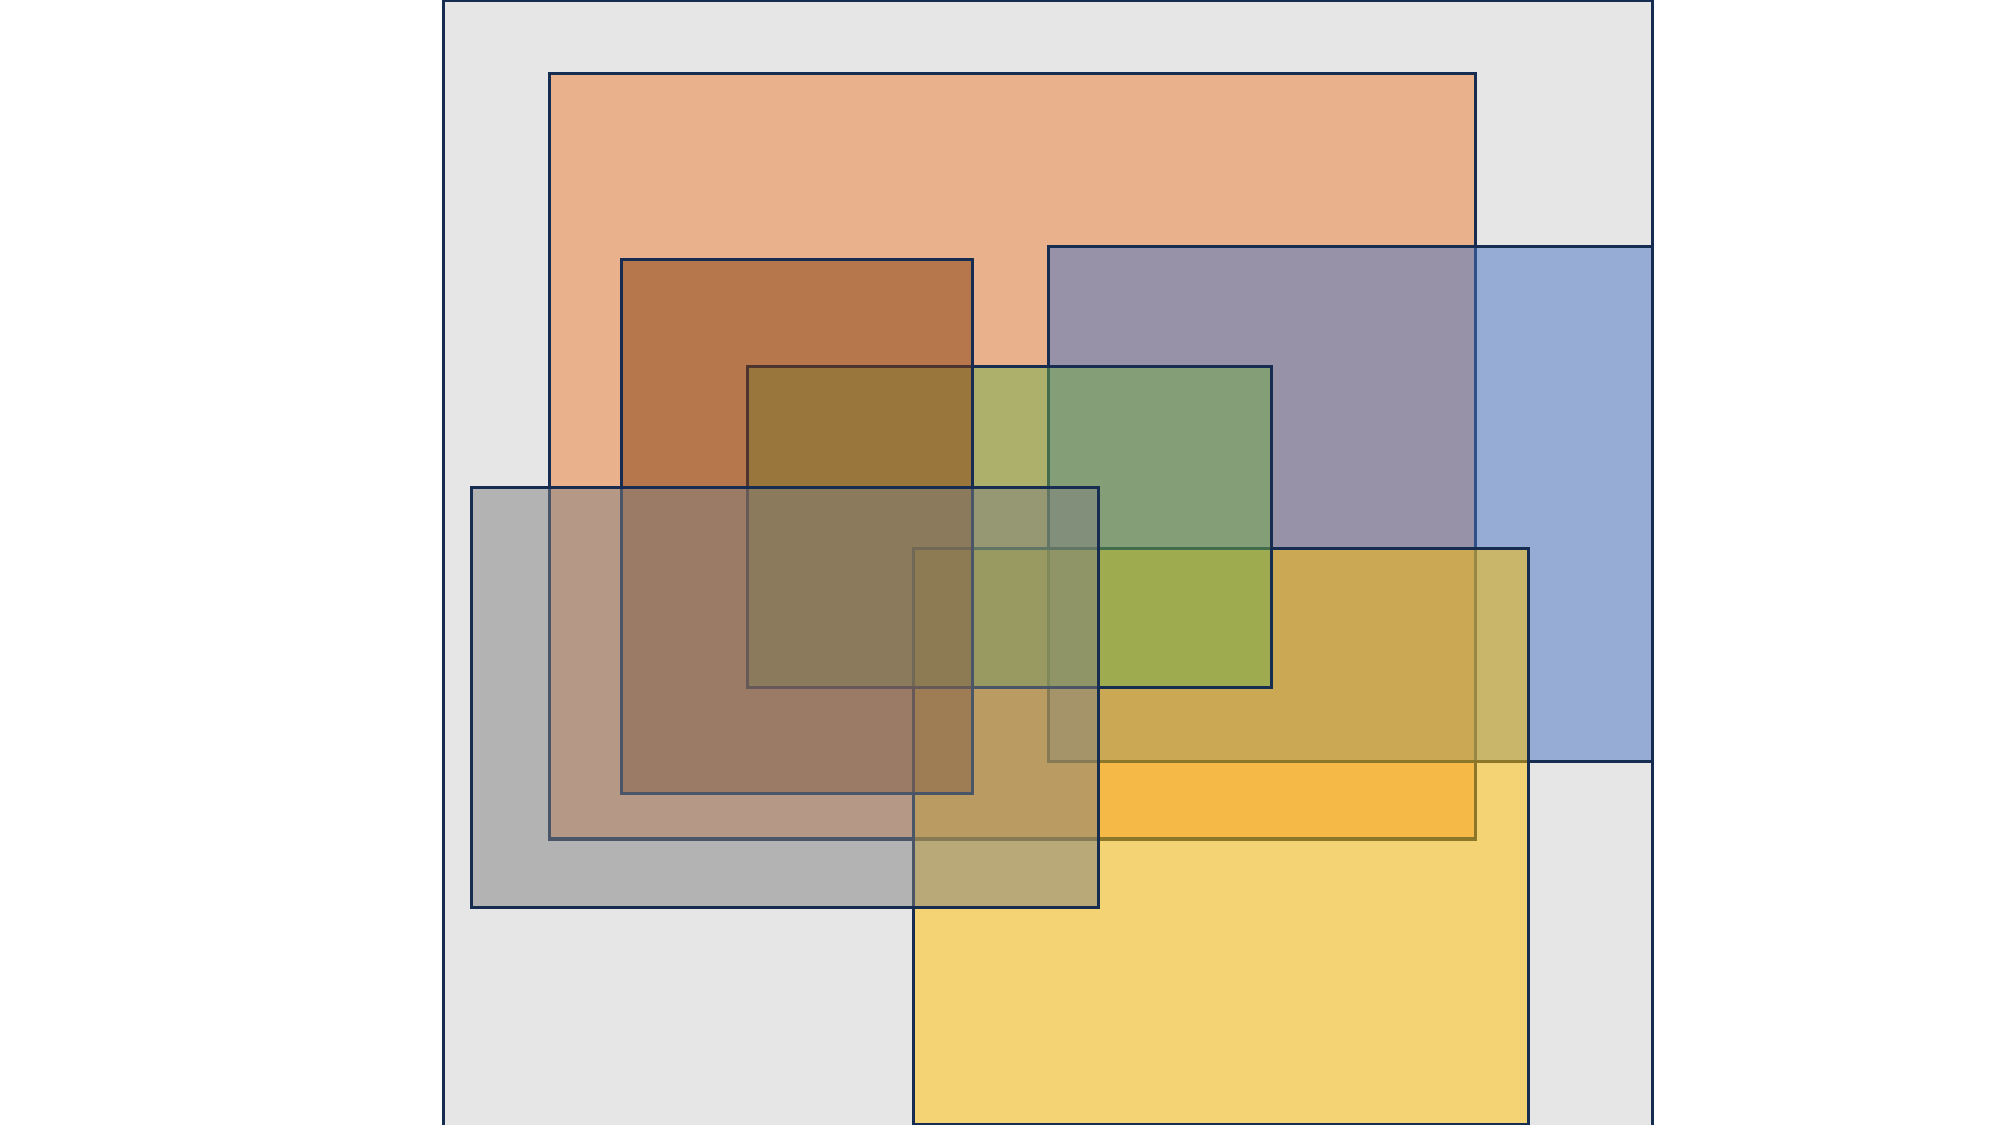
\includegraphics[width=0.8\textwidth]{figures/space-partition.pdf}
      \caption{How small changes lead to significant impacts.}
      \end{figure}
    \vspace{-1cm}

    \end{block}
  \begin{block}{\Large{\textbf{Bottleneck lies in BDD package.}}}
  \large
  The scalability of DPV systems is restricted by the scalability of BDD operations for two reasons: 

  \begin{enumerate}
    \item BDD operations contribute to the \efsz{majority of verification time}. Previous work 
    Flash have shown that BDD operations can account for the majority of the verification time 
    (i.e., the number of BDD operations reaches the order of $O(10^9)$ and 
    takes over 99\% of the overall time).

    \item Many parallelizable processes are hindered due to the \efsz{absence of parallelism support}.
    In cases of thread-safe packages, they either adopt expensive synchronizations or unsuitable
    scheme. In root, existing BDD packages are \efsz{not designed for throughput}.
  \end{enumerate}

  \end{block}
  \end{column}
\separatorcolumnB
%%%%%%%%%%%%%%%%%%%%%%%%%%%%%%%%%%%%%%%%%%%
%Section 2 column 2
%%%%%%%%%%%%%%%%%%%%%%%%%%%%%%%%%%%%%%%%%%%
\begin{column}[T]{\colwidthB}
\begin{table}[]
  \center
  \scriptsize
  \caption{Publicly available BDD libraries.}
% \vspace{-1.38em}
  \label{tab:bdd-libs}
  \resizebox{\linewidth}{!}{
  \begin{tabular}{|c|c|c|c|c|c|}
    \hline
    \emph{Name}
    & \emph{Lang}
    & \emph{Thread-safe}
    & \emph{Scalability}
    & \emph{Synchronization}
    & \emph{Execution}
    \\\hline
    BuDDy~ & C/C++ & N & Poor & User-lock & RtC
    \\\hline
    CUDD~ & C++ & N & Poor & User-lock & RtC
    \\\hline
    JDD~ & Java & N & Poor & User-lock & RtC
    \\\hline
    BeeDeeDee~ & C++ & Y & Medium & Mutex-lock & RtC
    \\\hline
    PJBDD~ & Java & Y & Medium & Lock-free & FJ
    \\\hline
    Sylvan~ & C++ & Y & Medium & Lock-free & FJ
    \\\hline
    HermesBDD~ & C++ & Y & High & Lock-free & FJ
    \\\hline
    \system & C++ & Y & High & Lock-free & RtC
    \\\hline
  \end{tabular}
  }
% \vspace{-2.88em}
\end{table}

\begin{block}{\Large{\textbf{Designs of Throughput-Optimized BDD}}}
  \vspace{0.5cm}
  \large
  \system is designed to achieve high throughput parallel BDD operations 
  by leveraging the multi-core capabilities of modern hardware.
  \begin{itemize}

    \item {\efsz{Reschedulable Thread-pool} to eliminate the overhead of frequent 
    thread creation and destruction, }

    \item {\efsz{Lock-free Node Table and Cache}. Inside it leverages CAS to achieve lock-free
    and dynamic linked lists to avoid resizing}

    \item {\efsz{Run-to-Completion} to avoid the overhead of interruption.}

    \item {\efsz{Commutative Hash Function} to reduce cache misses.}

  \end{itemize}
  % \large $\Rightarrow$ \textbf{\color{purple}{Detection}} 
\end{block}

\vspace{-0.5cm}
\begin{block}{\Large{\textbf{Use case: Scaling DPV with TOBDD}}}
\vspace{0.9cm}
\large
We implement \system~\footnote{https://github.com/guodong/tobdd} and 
a throughput-optimized version of Flash called TOFlash in C++. 
We compare the data plane model construction time of TOFlash with 
our previously implemented Flash artifact on various datasets.
\Cref{fig:eval} shows the evaluation results. We can see that 
\end{block}

\begin{figure}
\centering
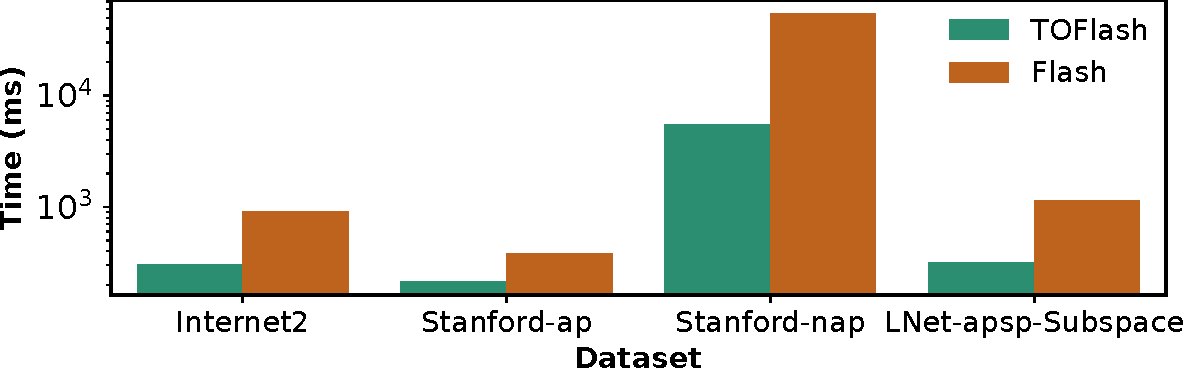
\includegraphics[width=1\textwidth]{figures/toflash.pdf}
\caption{TOFlash achieves 2-10x improvement compared with the baseline.}
\label{fig:eval}
\end{figure}

\end{column}
\separatorcolumnB
\end{columns}



\begin{columns}[t]
\begin{column}{\paperwidth}
\begin{figure}
\centering
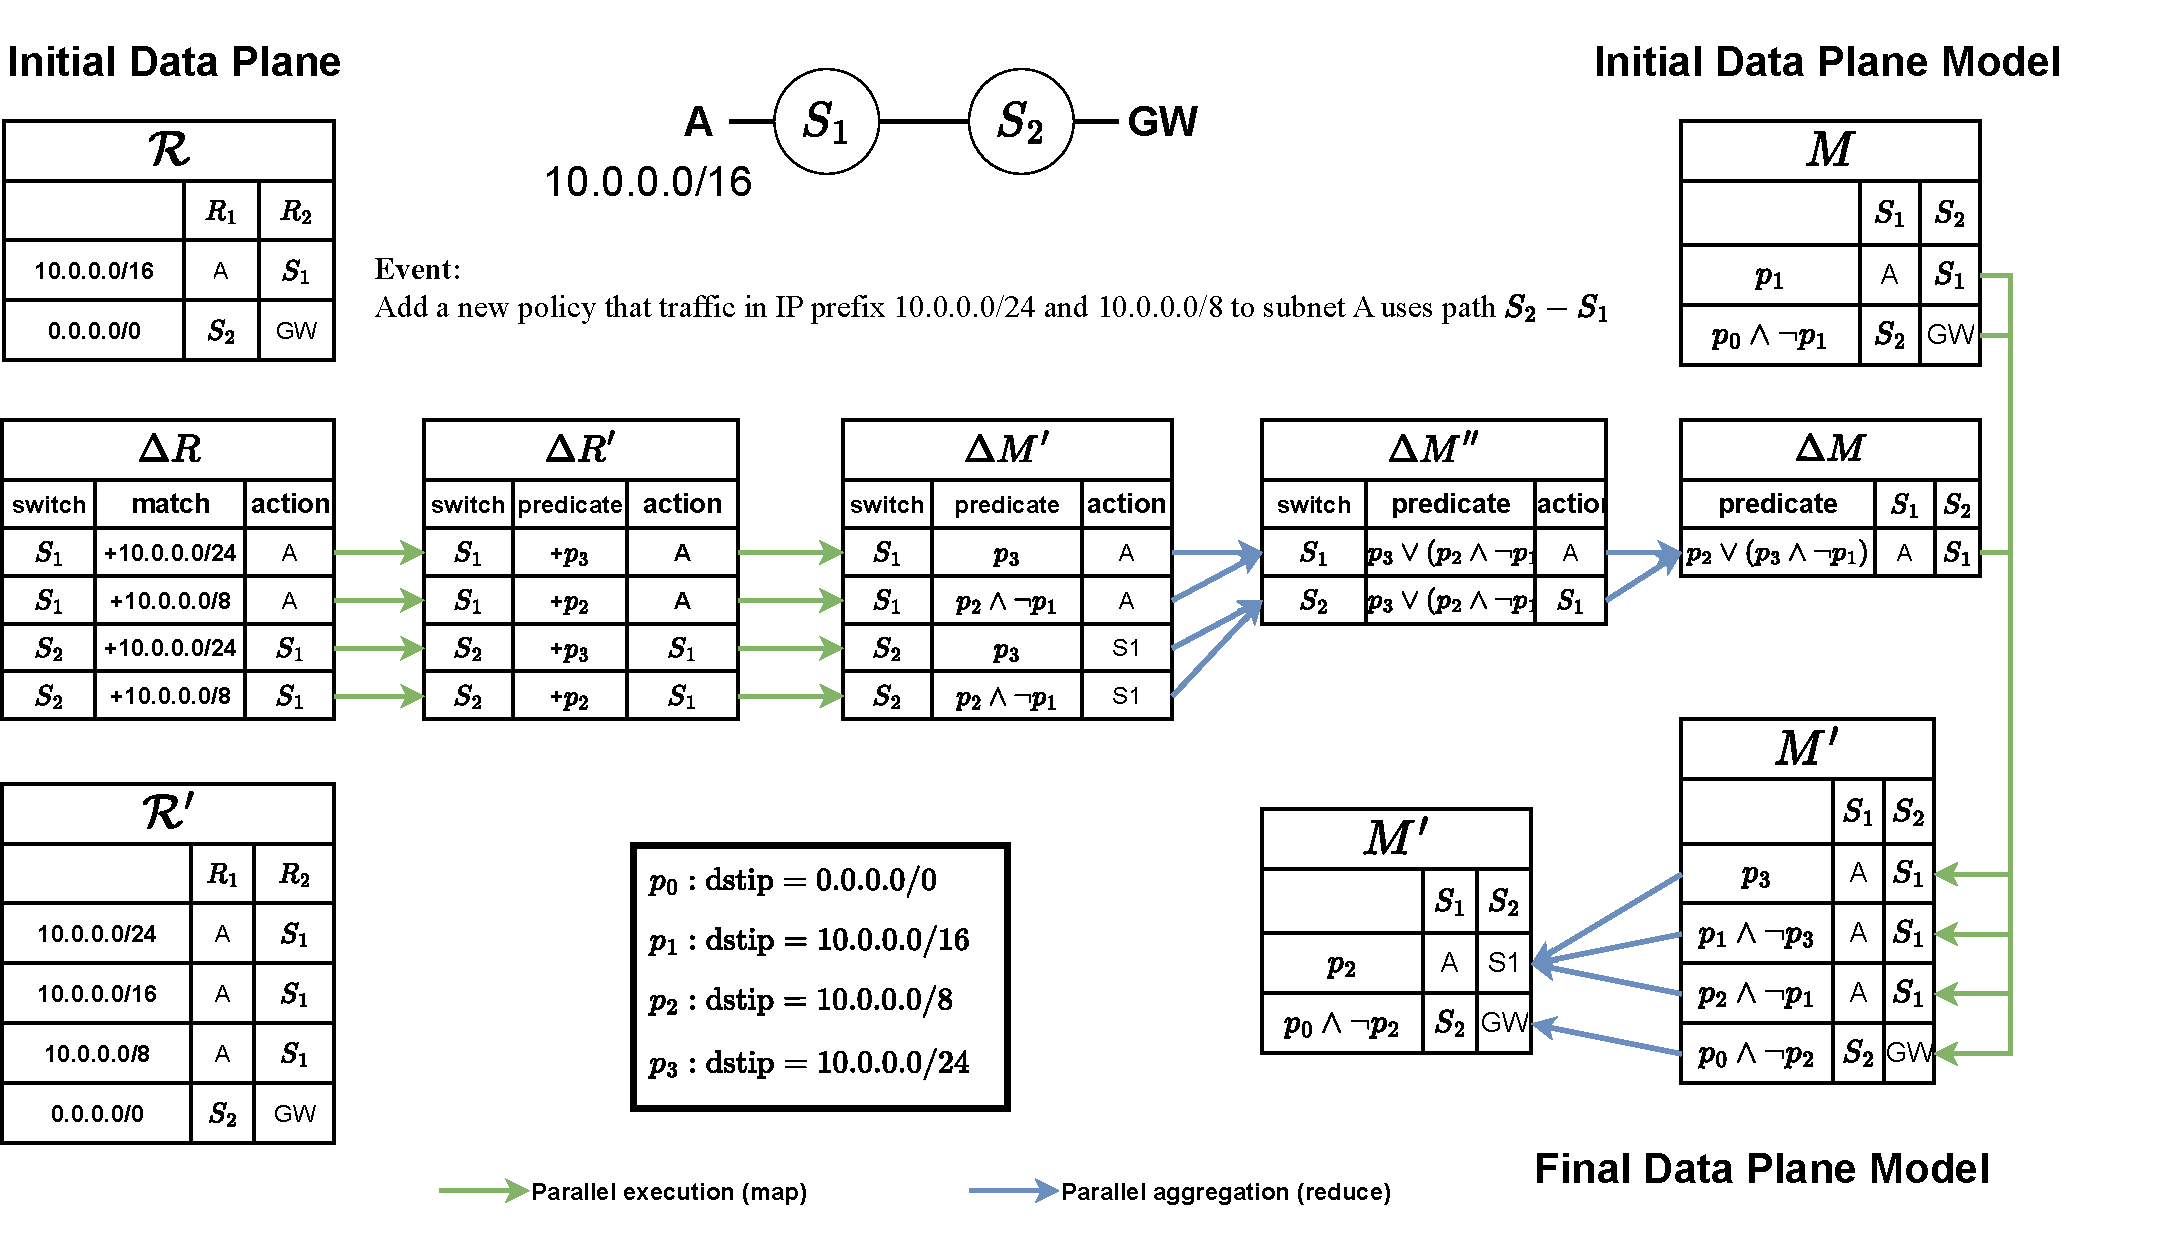
\includegraphics[width=0.8\paperwidth]{figures/example.pdf}
\caption{An example of ustilizing parallelism in DPV}
\end{figure}
\end{column}
\end{columns}

\end{frame}
\end{document}
